\chapter{Aprendizaje Reforzado}

\section{Or\'igenes y Descripci\'on}

Su principio se basa en la psicolog\'ia conductista: un \textit{agente} busca ser recompensado por un premio, el cual obtiene cuando realiza una secuencia de \textit{acciones} que lo llevan a concluir una tarea exitosamente. Adem\'as, para maximizar la cantidad de \textit{recompensa} que recibe - o, alternativamente, minimizar el tiempo que espera entre un premio y el siguiente - comienza a optimizar su pol\'itica (\textit{$\pi$}) para llegar a la meta satisfactoriamente. Una explicaci\'on mucho m\'as profunda de las bases e historia del aprendizaje reforzado, as\'i como la mayor parte de las definiciones mencionadas en este cap\'itulo, pueden ser encontradas en \citet{Sutton}.\\

\subsection{Terminolog\'ia com\'un}

Existen conceptos utilizados en pr\'acticamente la totalidad de los algoritmos de aprendizaje reforzado, independientemente de las particularidades que presenten. A continuaci\'on se presenta una lista, basada en la recopilaci\'on de \citet{rlexplained} no exhaustiva de ellos, pero que cubre los t\'erminos utilizados en este trabajo. La relaci\'on entre estos conceptos se puede consultar en la figura \ref{rl_concepts}, popularizada por \cite{Sutton}.

\begin{enumerate}
    \item Agente: es el concepto m\'as abstracto, pues es la entidad que aprender\'a durante el proceso. Por ejemplo, puede ser un rat\'on rob\'otico aprendiendo a llegar al queso en el laberinto; o un jugador virtual aprendiendo a superar todos los niveles de un videojuego.
    \item Estado: describe la situaci\'on en la cual se encuentra el agente. Por ejemplo, para el rat\'on rob\'otico, el estado es la casilla en la que se encuentra. El estado puede tener tantas dimensiones como sea necesario: por ejemplo, el estado de un coche autodirigido ser\'ia descrito por su posici\'on, velocidad, objetos en su radar e incluso cantidad de gasolina en el tanque.
    \item Mundo: se refiere la totalidad de los posibles estados.
    \item Acci\'on: es lo que un agente puede hacer en cada estado. Generalmente, el conjunto de acciones que puede tomar un agente en un estado determinado es finito, aunque el conjunto de acciones que tome durante todo el tiempo pueda tener combinaciones que se aproximen a infinito. Por ejemplo, para el rat\'on rob\'otico, sus acciones son realizar un movimiento hacia adelante, atr'as, derecha o izquierda.
    \item Recompensa: cuando un agente toma una acci\'on en un estado, recibe una recompensa. Es muy importante notar que la recompensa puede tomar muchas formas: es posible que sea solamente la meta \'ultima en vez de existir despu\'es de cada acci\'on (como el queso para el rat\'on). La recompensa tambi\'en puede ser negativa, equivalente a un castigo, lo cual causa que el agente aprenda a evitar las acciones que lo llevan a ella.
    \item Pol\'itica (\textit{policy}) es una funci\'on que toma como argumento un estado $s$ y devuelve una acci\'on $a$; equivalente a la estrategia del agente. La meta del aprendizaje reforzado es encontrar la pol\'itica \'optima. Generalmente se le representa como $\pi(s)->a$.
\end{enumerate}

\begin{figure}[ht]
\caption{Interacci\'on de los conceptos en Aprendizaje Reforzado}
\label{rl_concepts}
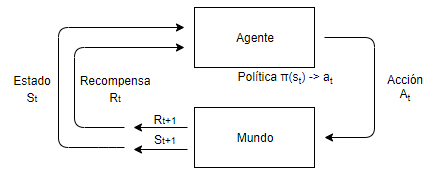
\includegraphics[width=10cm]{rl_concepts.PNG}
\centering
\end{figure}

Una vez que tenemos asignados estos elementos, resulta relativamente simple explicar el problema, pero no as\'i la implementaci\'on. Por ejemplo, para el rat\'on solamente recibir\'a la recompensa despu\'es de un movimiento espec\'ifico que lo lleve a la casilla en la que se encuentra el queso, todos los dem\'as movimientos son solamente un medio para acercarse. El aprendizaje reforzado resuelve esta situaci\'on asign\'andole valor a las recompensas a largo plazo en vez de solamente las inmediatas. Esto quiere decir que si planteamos el objetivo del aprendizaje como llegar al queso, el rat\'on no podr\'a decidir si es mejor un camino m\'as r\'apido o uno en el que dio vueltas sin sentido en un mismo lugar, siempre que en un tiempo finito haya llegado al centro. Sin embargo, acorde con la filosof\'ia del aprendizaje reforzado, si descontamos el valor del queso por cada casilla extra que le toma llegar a \'el, entonces buscar\'a el camino m\'as corto, optimizando su secuencia de acciones interactuando con el mundo que lo rodea para descubrir relaciones acci\'on-estado.\\

La principal caracter\'istica del agente es que tiene la capacidad de tomar decisiones sobre sus acciones, las cuales son su forma de interactuar con el mundo, llev\'andolo de un estado a otro. El agente no tiene acceso a todas las consecuencias de sus acciones; de hecho, ni siquiera conoce todo el mundo.\\

El agente toma una acci\'on en el tiempo $t$, la cual depende del estado $s_t$ del mundo. En $t+1$, el mundo reaccion\'o ya a la interacci\'on del agente con \'el, as\'i que el agente recibe una recompensa $r_{t+1}$ y toma una nueva acci\'on dependiendo del estado $s_{t+1}$ del mundo. Sin embargo, no es \'optimo seleccionar acciones solamente con base en la recompensa $r_{t+1}$, pues la naturaleza temporal del problema lo convierte en un problema a largo plazo, y el agente estar\'ia considerando solamente consecuencias en el corto plazo.\\

As\'i, el agente debe aprender que existe un \textit{retraso} entre cada acci\'on que toma y el premio. Supongamos que, en una cuadr\'icula, el premio se encuentra en la casilla (x,y). El agente solamente puede llegar a esa casilla meta desde las adyacentes, pero si no se encuentra en una de estas, primero debe acercarse a alguna de las casillas adyacentes, por ejemplo (x-1,y). Recursivamente, si no se encuentra en ninguna de estas casillas, debe encontrar un camino que lo lleve ah\'i. Este proceso se conoce como \textit{exploraci\'on}, pues es posible que el agente no reciba ninguna recompensa por sus acciones hasta que encuentre por primera vez la casilla (x,y) en en tiempo \textit{t} y asigne un valor de recompensa positivo (aunque descontado) a la casilla en la que se encontraba al tiempo \textit{t-1}. As\'i, cuando el agente comienza su exploraci\'on, ir\'a aprendiendo que, lejos de que la recompensa sea inmediata, debe tomar una secuencia de acciones para llegar a ella. Una vez que el agente tiene mejor conocimiento acerca de cu\'ales casillas lo acercan al premio, pasa a una fase llamada \textit{explotaci\'on}, en la cual busca la recompensa m\'as grande entre todas las que conoce. Un agente debe comenzar su aprendizaje puramente en modo explotatorio, y transicionar al modo de explotaci\'on conforme conoce mejor su ambiente.\\

Podemos entonces definir la \textit{funci\'on de valor} asociada a la pol\'itica como el valor esperado de la recompensa al tiempo $t$ dado que el agente se encuentra en el estado $s$. Adem\'as, cada periodo de tiempo se le aplica un factor de descuento $\gamma$ para obtener el valor presente de tal recompensa. De esta definici\'on deriva uno de los conceptos m\'as importantes en el aprendizaje reforzado, la \textit{Ecuaci\'on de Bellman}. A continuaci\'on se presenta el desarrollo de \'esta. \\

La idea b\'asica es que la recompensa en el tiempo $t$ es:

\vspace{-30pt}
\begin{align*}
R_{t} &= r_{t+1} + \gamma r_{t+2} + \gamma^{2} r_{t+3} + \gamma^{3} r_{t+4} + ... \\
R_{t} &= r_{t+1} + \gamma \left( r_{t+2} + \gamma r_{t+3} + \gamma^{2}r_{t+4} + ...  \right)  \\
R_{t} &= r_{t+1} + \gamma R_{t+1}
\end{align*}

El valor de un estado $s$ se puede definir como la recompensa esperada dado que el agente empieza en ese estado, y depende de su pol\'itica:

$$
V^{\pi}(s) = E_{\pi}\left\{R_{t}|s_{t} = s\right\} = E_{\pi}\left\{\sum_{k=0}^{\infty}\gamma^{k}r_{t+k+1}|s_{t}=s\right\}
$$

Tambi\'en es necesario que el agente ajuste su comportamiento mientras transcurre el tiempo: al principio debe explorar para conocer la mayor cantidad de consecuencias a sus acciones posibles, pero m\'as adelante debe mantener el conocimiento de cu\'ales acciones le han reportado buenas acciones y tomar esas decisiones m\'as seguido. A esta estrategia de exploraci\'on se le llama $\epsilon-greedy$.\\

Definamos $p_r{t}$ y $p_t{t}$ como las probabilidades al tiempo $t$ de exploraci\'on y explotaci\'on, respectivamente. Entonces:

\vspace{-30pt}
\begin{align*}
p_r{t} &= 1 - \epsilon(t) \\
p_t{t} &= 1 - p_r{t} \quad \quad \forall t
\end{align*}

La funci\'on $\epsilon$ suele ser implementada como decreciente de forma lineal para el aprendizaje,  de tal forma que mientras pasa el tiempo, el agente escoge las acciones conocidas que le reportan mayor utilidad m\'as seguido; junto con un par\'ametro $\rho$ aleatorio para asegurar que siempre existe una probabilidad positiva de explorar.\\

Generalmente se supone este tipo de problemas como Procesos de Decisi\'on de Markov (MDP), cuya principal caracter\'istica es que cumplen con la famosa propiedad de Markov: a grandes rasgos, el futuro solamente depende del presente, no del pasado.\\

Formalmente, un proceso de Markov es una tupla $(X,U,f,\rho)$ en donde $X$ es el conjunto finito de estados, $U$ es el conjunto finito de aciones de un agente, $f:X*U*X\rightarrow[0,1]$ es la funci\'on de probabilidad de transici\'on de estado, y $\rho:X*U*X\rightarrow\mathbb{R}$ es la funci\'on de recompensa. \\

Cuando el conjunto de acciones (o el \textit{policy}) a tomar es dif\'icil de aprender porque no existen ejemplos, o el mundo / conjunto de acciones / conjunto de consecuencias es demasiado grande, es apropiado utilizar Aprendizaje Reforzado en lugar de Aprendizaje de M\'aquina regular. Gracias a que el agente va descubriendo y acerc\'andose a una pol\'itica \'optima, no es necesario que explore todas las acciones posibles. \\

En este trabajo se aplicar\'an dos algoritmos sumamente conocidos y aplicados en un sinf\'in de \'ambitos: \textit{Policy Iteration} y \textit{Q-learning}, y compararemos su rendimiento al aplicarlos al problema de la distribuci\'on de cerveza.

\section{Policy Iteration}

En este algoritmo, se empieza con una pol\'itica aleatoria, se encuentra el valor de ella, y se realiza un paso que encuentra una pol\'itica nueva (mejor) basado en la anterior. De esta manera, \textit{policy iteration} asegura convergencia a la pol\'itica \'optima. \\

La ecuaci\'on que representa este algoritmo es:

$$
\pi_0 \overset{E}{\rightarrow} V^{\pi_{0}} \overset{I}{\rightarrow}
\pi_1 \overset{E}{\rightarrow} V^{\pi_{1}} \overset{I}{\rightarrow}
\pi_2 \overset{E}{\rightarrow} 
...
\overset{I}{\rightarrow} \pi_{*} \overset{I}{\rightarrow} V^{\pi_{*}}
$$

En donde $\overset{E}{\rightarrow}$ significa que una pol\'itica se \textit{eval\'ua}, y $\overset{I}{\rightarrow}$ significa que se mejora (por \textit{improvement}, en ingl\'es). \\

Se suele preferir este algoritmo sobre \textit{value iteration}, pues es com\'un que se encuentre la pol\'itica \'optima mucho antes de que la funci\'on de valor converja. Adem\'as, dado que se itera sobre la pol\'itica anterior y se busca una mejor, el algoritmo converge r\'apidamente y cada paso asegura una mejora.

\section{Q-Learning}

Uno de los algoritmos m\'as populares de aprendizaje es \textit{Q-learning}. Obtiene este nombre por la \textit{funci\'on Q}, la cual indica el valor descontado de la recompensa asociado a una acci\'on en un estado determinado.

\subsection{Conceptos}

Recordemos la ecuaci\'on de valor de un estado, basada en la ecuaci\'on de Bellman, que fue desarrollada en la secci\'on introductoria:

$$
V^{\pi}(s) = E_{\pi}\left\{R_{t}|s_{t} = s\right\} = E_{\pi}\left\{\sum_{k=0}^{\infty}\gamma^{k}r_{t+k+1}|s_{t}=s\right\}
$$

De aqu\'i sigue que el valor de tomar una acci\'on espec\'ifica $a$ en el estado $s$ usando la pol\'itica $\pi$ es:

$$
    Q_{\pi}(s,a) = E_{\pi}\left\{R_{t}|s_{t}=s,a_{t}=a\right\}=E_{\pi}\left \{\sum_{k = 0}^{\infty}\gamma^{k}r_{t+k+1}|s_{t} =s, a_{t} =a  \right \}
$$

%aqui se pone la definicion de Q
$$
V(s) = \max_{a}{Q(s,a)}
$$
$$
Q(s, a) = R(s, a) + \gamma * \max_{a}{Q(s^{'}, a^{*})}
$$

Donde $s{'}$ es el siguiente estado, y $a^{*}$ representa todas las acciones posibles. Al estimar la funci\'on $Q$ para cada par de estado con acci\'on, es posible encontrar la mejor acci\'on para cada estado y, as\'i, obtener una pol\'itica \'optima.\\

Al iniciar el periodo de aprendizaje del algoritmo, la funci\'on Q se establece como $Q(s,a) = 0 \; \forall \; s, a$, y en cada paso (e iteraci\'on) se actualiza su valor.

\subsection{Algoritmo}

\begin{enumerate}
    \item Asignar $Q(s,a) = 0$ para todos los estados y acciones.
    \item Posicionarse en un estado $s$
    \item Seleccionar acci\'on $a^{*}$ y ejecutar
    \item Recibir recompensa $r$
    \item Observar estado nuevo $s^{'}$
    \item Actualizar $\hat{Q}(s,a) = r(s,a) + \lambda \max _{ a^{'} }{  \hat{Q}(s^{'},a^{'}) }$
    \item Asignar nuevo estado $s \leftarrow s^{'}$
    \item Volver a 2 hasta convergencia
\end{enumerate}

Hasta este momento, hemos establecido las bases para dos t\'ecnicas de aprendizaje reforzado para un agente. Sin embargo, el Problema de la Distribución de Cerveza es multiagente por naturaleza: cada eslab\'on de la cadena de suministro juega un papel diferente o puede tener m\'argenes y costos diferentes. Esta generalizaci\'on se conoce como Aprendizaje Reforzado Multi-Agente, el cual presenta retos nuevos, al tiempo de abrir las puertas a sistemas din\'amicos m\'as complejos.

\section{Aprendizaje Reforzado Multi-Agente (ARM)}

Existen muchos problemas que inherentemente parecen tener soluciones sencillas, pero es necesario que m\'as de un agente aprenda de manera simult\'anea, especialemnte si la recompensa al final es compartida entre todos ellos. Por ejemplo, imaginemos que tenemos dos robots, ladrillos y un cuadro dibujado en el piso. Cada uno de los robots est\'a cerca de esquinas opuestas y tiene acceso a la mitad de los ladrillos. La recompensa final se les otorga cuando forman un cuadrado de ladrillos, y es mayor mientras menor sea el tiempo que les tome terminar. En este caso, la estrategia \'optima es que cada uno de los robots coloque, en cada tiempo, el ladrillo que m\'as cerca le quede. El probema se vuelve sumamente complejo, pues cambios en la estrategia de un agente puedem afectar la estrategia de otros agentes. Por ejemplo, si uno de los robots tiene un comportamiento err\'atico porque recibe un castigo si le sobra energ\'ia al terminar la tarea, el otro deber\'a adaptarse a esta nueva forma de actuar.\\

A grandes rasgos el aprendizaje reforzado multiagente (ARM), es una generalizaci\'on de los conceptos estudiados anteriormente, al permitir m\'as de un agente aprender y tomar sus propias decisiones, en un mundo en el cual puede interactuar con los dem\'as. Muchas de las definiciones espec\'ificas del ARM, as\'i como de su intersecci\'on con teor\'ia de juegos, pueden encontrarse en \citet{Bloembergen}. \\

Existen pros y contras relacionados al ARM, como los referidos por \citet{Busoniu}. Algunos beneficios son que es posible que algunos agentes asuman tareas ajenas si esto ayuda a la optimizaci\'on del premio final, es inherentemente rubusto, y generalmente est\'an dise\~nados de tal manera que a\~nadir nuevos agentes es f\'acil. Por otro lado, algunos retos son la escalabilidad debido al crecimiento exponencial de la dimensi\'on del espacio estado-acci\'on, o a la complejidad que se genera al a\~nadir cada nuevo agente.\\

En este trabajo, se considerar\'a a cada eslab\'on de la cadena de suministro de cerveza como un agente. Cada agente solamente puede comunicarse con los niveles inmediatamente vecinos; es decir, las \'unicas interacciones que puede tener con el mundo son el n\'umero de \'ordenes que recibe del nivel inferior y el inventario que pide al nivel superior. De esta manera, nuestros agentes no son adversarios, cooperativos ni independientes; esto es un \textit{input} de la direcci\'on en la cual fluye la cadena de suministro. El objetivo de cada agente es maximizar sus recompensas individuales.\\

Hemos definido una penalizaci\'on por mantener cerveza en el inventario (el costo del almac\'en), as\'i que la decisi\'on concerniente a la petici\'on del nivel inferior queda determinada: vender\'a todo lo que pueda, pues cada venta le reporta una ganancia, y no llenar la orden completa cuando tiene suficiente inventario lo har\'ia incurrir en un costo innecesario (esto, por supuesto, podr\'ia ser otro \textit{policy}).\\

Para cada agente, el conjunto de \textbf{acciones} que puede tomar es solamente el n\'umero de cervezas que pedir\'a al nivel inmediatamente superior en cada tiempo $t$. Lo que tendr\'a guardado en la bodega en el tiempo $t$ estar\'a constituido por el n\'umero de cervezas que ten\'ia en el tiempo anterior $t-1$, menos el n\'umero de cervezas vendidas al agente inferior, m\'as el n\'umero de cervezas que recibe del nivel inmediatamente superior por el pedido de reaprovisionamiento, restringido a que cada agente solamente cubrir\'a la orden del nivel inferior si tiene suficiente inventario para hacerlo.\\

El objetivo de cada agente es maximizar su recompensa. Sin embargo, este es un problema ligeramente diferente a los comunes de \textit{Q-learning}, en los cuales el valor de la recompensa es conocido y, una vez encontrado, se buscan las acciones \'optimas ``de atr\'as hacia adelante'' (como el ejemplo antes mencionado de un rat\'on buscando un queso en un laberinto).\\

Su pol\'itica est\'a definida con base en la funci\'on Q, una vez que el proceso de aprendizaje fue finalizado, de esta manera, puede realizar una b\'usqueda sobre todas las posibles acciones en los estados y sencillamente escoger la mejor, lo cual converge a la pol\'itica (cuasi)\'optima. \\

Es importante destacar que este sistema toma solamente una de las ramas que existen en la industria de cualquier producto (existe m\'as de un minorista, etc.), e incluso, toma solamente un producto. Es entonces una generalizaci\'on en la que se propone un ``agente representativo'' en cada nivel de la cadena. A\'un as\'i, es un sistema complejo bastante robusto y sensible a cambios peque\~nos como un aumento en el costo de almacenaje o un cambio agresivo en el margen de un eslab\'on.

